% Options for packages loaded elsewhere
% Options for packages loaded elsewhere
\PassOptionsToPackage{unicode}{hyperref}
\PassOptionsToPackage{hyphens}{url}
%
\documentclass[
  ignorenonframetext,
]{beamer}
\newif\ifbibliography
\usepackage{pgfpages}
\setbeamertemplate{caption}[numbered]
\setbeamertemplate{caption label separator}{: }
\setbeamercolor{caption name}{fg=normal text.fg}
\beamertemplatenavigationsymbolsempty
% remove section numbering
\setbeamertemplate{part page}{
  \centering
  \begin{beamercolorbox}[sep=16pt,center]{part title}
    \usebeamerfont{part title}\insertpart\par
  \end{beamercolorbox}
}
\setbeamertemplate{section page}{
  \centering
  \begin{beamercolorbox}[sep=12pt,center]{section title}
    \usebeamerfont{section title}\insertsection\par
  \end{beamercolorbox}
}
\setbeamertemplate{subsection page}{
  \centering
  \begin{beamercolorbox}[sep=8pt,center]{subsection title}
    \usebeamerfont{subsection title}\insertsubsection\par
  \end{beamercolorbox}
}
% Prevent slide breaks in the middle of a paragraph
\widowpenalties 1 10000
\raggedbottom
\AtBeginPart{
  \frame{\partpage}
}
\AtBeginSection{
  \ifbibliography
  \else
    \frame{\sectionpage}
  \fi
}
\AtBeginSubsection{
  \frame{\subsectionpage}
}
\usepackage{iftex}
\ifPDFTeX
  \usepackage[T1]{fontenc}
  \usepackage[utf8]{inputenc}
  \usepackage{textcomp} % provide euro and other symbols
\else % if luatex or xetex
  \usepackage{unicode-math} % this also loads fontspec
  \defaultfontfeatures{Scale=MatchLowercase}
  \defaultfontfeatures[\rmfamily]{Ligatures=TeX,Scale=1}
\fi
\usepackage{lmodern}

\usetheme[]{CambridgeUS}
\usefonttheme[]{professionalfonts}
\ifPDFTeX\else
  % xetex/luatex font selection
\fi
% Use upquote if available, for straight quotes in verbatim environments
\IfFileExists{upquote.sty}{\usepackage{upquote}}{}
\IfFileExists{microtype.sty}{% use microtype if available
  \usepackage[]{microtype}
  \UseMicrotypeSet[protrusion]{basicmath} % disable protrusion for tt fonts
}{}
\makeatletter
\@ifundefined{KOMAClassName}{% if non-KOMA class
  \IfFileExists{parskip.sty}{%
    \usepackage{parskip}
  }{% else
    \setlength{\parindent}{0pt}
    \setlength{\parskip}{6pt plus 2pt minus 1pt}}
}{% if KOMA class
  \KOMAoptions{parskip=half}}
\makeatother

\usepackage{color}
\usepackage{fancyvrb}
\newcommand{\VerbBar}{|}
\newcommand{\VERB}{\Verb[commandchars=\\\{\}]}
\DefineVerbatimEnvironment{Highlighting}{Verbatim}{commandchars=\\\{\}}
% Add ',fontsize=\small' for more characters per line
\usepackage{framed}
\definecolor{shadecolor}{RGB}{241,243,245}
\newenvironment{Shaded}{\begin{snugshade}}{\end{snugshade}}
\newcommand{\AlertTok}[1]{\textcolor[rgb]{0.68,0.00,0.00}{#1}}
\newcommand{\AnnotationTok}[1]{\textcolor[rgb]{0.37,0.37,0.37}{#1}}
\newcommand{\AttributeTok}[1]{\textcolor[rgb]{0.40,0.45,0.13}{#1}}
\newcommand{\BaseNTok}[1]{\textcolor[rgb]{0.68,0.00,0.00}{#1}}
\newcommand{\BuiltInTok}[1]{\textcolor[rgb]{0.00,0.23,0.31}{#1}}
\newcommand{\CharTok}[1]{\textcolor[rgb]{0.13,0.47,0.30}{#1}}
\newcommand{\CommentTok}[1]{\textcolor[rgb]{0.37,0.37,0.37}{#1}}
\newcommand{\CommentVarTok}[1]{\textcolor[rgb]{0.37,0.37,0.37}{\textit{#1}}}
\newcommand{\ConstantTok}[1]{\textcolor[rgb]{0.56,0.35,0.01}{#1}}
\newcommand{\ControlFlowTok}[1]{\textcolor[rgb]{0.00,0.23,0.31}{\textbf{#1}}}
\newcommand{\DataTypeTok}[1]{\textcolor[rgb]{0.68,0.00,0.00}{#1}}
\newcommand{\DecValTok}[1]{\textcolor[rgb]{0.68,0.00,0.00}{#1}}
\newcommand{\DocumentationTok}[1]{\textcolor[rgb]{0.37,0.37,0.37}{\textit{#1}}}
\newcommand{\ErrorTok}[1]{\textcolor[rgb]{0.68,0.00,0.00}{#1}}
\newcommand{\ExtensionTok}[1]{\textcolor[rgb]{0.00,0.23,0.31}{#1}}
\newcommand{\FloatTok}[1]{\textcolor[rgb]{0.68,0.00,0.00}{#1}}
\newcommand{\FunctionTok}[1]{\textcolor[rgb]{0.28,0.35,0.67}{#1}}
\newcommand{\ImportTok}[1]{\textcolor[rgb]{0.00,0.46,0.62}{#1}}
\newcommand{\InformationTok}[1]{\textcolor[rgb]{0.37,0.37,0.37}{#1}}
\newcommand{\KeywordTok}[1]{\textcolor[rgb]{0.00,0.23,0.31}{\textbf{#1}}}
\newcommand{\NormalTok}[1]{\textcolor[rgb]{0.00,0.23,0.31}{#1}}
\newcommand{\OperatorTok}[1]{\textcolor[rgb]{0.37,0.37,0.37}{#1}}
\newcommand{\OtherTok}[1]{\textcolor[rgb]{0.00,0.23,0.31}{#1}}
\newcommand{\PreprocessorTok}[1]{\textcolor[rgb]{0.68,0.00,0.00}{#1}}
\newcommand{\RegionMarkerTok}[1]{\textcolor[rgb]{0.00,0.23,0.31}{#1}}
\newcommand{\SpecialCharTok}[1]{\textcolor[rgb]{0.37,0.37,0.37}{#1}}
\newcommand{\SpecialStringTok}[1]{\textcolor[rgb]{0.13,0.47,0.30}{#1}}
\newcommand{\StringTok}[1]{\textcolor[rgb]{0.13,0.47,0.30}{#1}}
\newcommand{\VariableTok}[1]{\textcolor[rgb]{0.07,0.07,0.07}{#1}}
\newcommand{\VerbatimStringTok}[1]{\textcolor[rgb]{0.13,0.47,0.30}{#1}}
\newcommand{\WarningTok}[1]{\textcolor[rgb]{0.37,0.37,0.37}{\textit{#1}}}

\usepackage{longtable,booktabs,array}
\usepackage{calc} % for calculating minipage widths
\usepackage{caption}
% Make caption package work with longtable
\makeatletter
\def\fnum@table{\tablename~\thetable}
\makeatother
\usepackage{graphicx}
\makeatletter
\newsavebox\pandoc@box
\newcommand*\pandocbounded[1]{% scales image to fit in text height/width
  \sbox\pandoc@box{#1}%
  \Gscale@div\@tempa{\textheight}{\dimexpr\ht\pandoc@box+\dp\pandoc@box\relax}%
  \Gscale@div\@tempb{\linewidth}{\wd\pandoc@box}%
  \ifdim\@tempb\p@<\@tempa\p@\let\@tempa\@tempb\fi% select the smaller of both
  \ifdim\@tempa\p@<\p@\scalebox{\@tempa}{\usebox\pandoc@box}%
  \else\usebox{\pandoc@box}%
  \fi%
}
% Set default figure placement to htbp
\def\fps@figure{htbp}
\makeatother





\setlength{\emergencystretch}{3em} % prevent overfull lines

\providecommand{\tightlist}{%
  \setlength{\itemsep}{0pt}\setlength{\parskip}{0pt}}



 


\usepackage{booktabs}
\usepackage{longtable}
\usepackage{array}
\usepackage{multirow}
\usepackage{wrapfig}
\usepackage{float}
\usepackage{colortbl}
\usepackage{pdflscape}
\usepackage{tabu}
\usepackage{threeparttable}
\usepackage{threeparttablex}
\usepackage[normalem]{ulem}
\usepackage{makecell}
\usepackage{xcolor}
\makeatletter
\@ifpackageloaded{tcolorbox}{}{\usepackage[skins,breakable]{tcolorbox}}
\@ifpackageloaded{fontawesome5}{}{\usepackage{fontawesome5}}
\definecolor{quarto-callout-color}{HTML}{909090}
\definecolor{quarto-callout-note-color}{HTML}{0758E5}
\definecolor{quarto-callout-important-color}{HTML}{CC1914}
\definecolor{quarto-callout-warning-color}{HTML}{EB9113}
\definecolor{quarto-callout-tip-color}{HTML}{00A047}
\definecolor{quarto-callout-caution-color}{HTML}{FC5300}
\definecolor{quarto-callout-color-frame}{HTML}{acacac}
\definecolor{quarto-callout-note-color-frame}{HTML}{4582ec}
\definecolor{quarto-callout-important-color-frame}{HTML}{d9534f}
\definecolor{quarto-callout-warning-color-frame}{HTML}{f0ad4e}
\definecolor{quarto-callout-tip-color-frame}{HTML}{02b875}
\definecolor{quarto-callout-caution-color-frame}{HTML}{fd7e14}
\makeatother
\makeatletter
\@ifpackageloaded{caption}{}{\usepackage{caption}}
\AtBeginDocument{%
\ifdefined\contentsname
  \renewcommand*\contentsname{Table of contents}
\else
  \newcommand\contentsname{Table of contents}
\fi
\ifdefined\listfigurename
  \renewcommand*\listfigurename{List of Figures}
\else
  \newcommand\listfigurename{List of Figures}
\fi
\ifdefined\listtablename
  \renewcommand*\listtablename{List of Tables}
\else
  \newcommand\listtablename{List of Tables}
\fi
\ifdefined\figurename
  \renewcommand*\figurename{Figure}
\else
  \newcommand\figurename{Figure}
\fi
\ifdefined\tablename
  \renewcommand*\tablename{Table}
\else
  \newcommand\tablename{Table}
\fi
}
\@ifpackageloaded{float}{}{\usepackage{float}}
\floatstyle{ruled}
\@ifundefined{c@chapter}{\newfloat{codelisting}{h}{lop}}{\newfloat{codelisting}{h}{lop}[chapter]}
\floatname{codelisting}{Listing}
\newcommand*\listoflistings{\listof{codelisting}{List of Listings}}
\makeatother
\makeatletter
\makeatother
\makeatletter
\@ifpackageloaded{caption}{}{\usepackage{caption}}
\@ifpackageloaded{subcaption}{}{\usepackage{subcaption}}
\makeatother

\usepackage{bookmark}
\IfFileExists{xurl.sty}{\usepackage{xurl}}{} % add URL line breaks if available
\urlstyle{same}
\hypersetup{
  pdftitle={Descubriendo Patrones con Frecuencias Simples},
  pdfauthor={Mario Morales},
  hidelinks,
  pdfcreator={LaTeX via pandoc}}


\title{Descubriendo Patrones con Frecuencias Simples}
\subtitle{Con datos de ejemplos de R}
\author{Mario Morales}
\date{2026-03-01}

\begin{document}
\frame{\titlepage}

\renewcommand*\contentsname{Table of contents}
\begin{frame}[allowframebreaks]
  \frametitle{Table of contents}
  \setcounter{tocdepth}{3}
  \tableofcontents
\end{frame}
\setcounter{tocdepth}{3}
\tableofcontents
}

\section{Fecha de la clase: Lunes 2 de marzo de
2026.}\label{fecha-de-la-clase-lunes-2-de-marzo-de-2026.}

\begin{frame}[fragile]{¿Qué haremos en clase?}
\phantomsection\label{quuxe9-haremos-en-clase}
Trabajaremos el tema {Distribuciones de Frecuencia Simples} para
variables discretas o con pocos valores, usaremos un conjunto de datos
clásico de \texttt{R} que resultará muy intuitivo y fácil de trabajar a
los estudiantes.
\end{frame}

\section{Ejemplo desarrolado por el profesor en
clase}\label{ejemplo-desarrolado-por-el-profesor-en-clase}

\begin{frame}[fragile]{El Problema: ¿Qué tan \texttt{familiares} son los
autos de los 70?}
\phantomsection\label{el-problema-quuxe9-tan-familiares-son-los-autos-de-los-70}
Utilizaremos el dataset \texttt{mtcars} ({Motor Trend Car Road Tests}.
Este dataset contiene información sobre el diseño y rendimiento de 32
automóviles (modelos 1973-74).
\end{frame}

\begin{frame}[fragile]{Planteamiento}
\phantomsection\label{planteamiento}
\begin{tcolorbox}[enhanced jigsaw, opacityback=0, titlerule=0mm, bottomtitle=1mm, colbacktitle=quarto-callout-important-color!10!white, title=\textcolor{quarto-callout-important-color}{\faExclamation}\hspace{0.5em}{Important}, toptitle=1mm, arc=.35mm, breakable, leftrule=.75mm, coltitle=black, toprule=.15mm, colframe=quarto-callout-important-color-frame, left=2mm, rightrule=.15mm, bottomrule=.15mm, colback=white, opacitybacktitle=0.6]

Imagina que eres un analista de mercado en 1974. Quieres entender la
configuración de los motores de la época, específicamente el
\textbf{número de carburadores (\texttt{carb})} que tienen los
vehículos, para identificar qué tan comunes eran los autos de alto
rendimiento versus los de uso diario.

\end{tcolorbox}
\end{frame}

\begin{frame}[fragile]{Plan de acción I}
\phantomsection\label{plan-de-acciuxf3n-i}
\begin{itemize}
\item
  \textbf{Exploración:} Cargar los datos y aislar la variable de interés
  (\texttt{carb}).
\item
  \textbf{Sintetizar:} Crear la tabla de frecuencias que incluya:

  \begin{itemize}
  \tightlist
  \item
    Frecuencia Absoluta (\(n_i\)).
  \item
    Frecuencia Absoluta Acumulada (\(N_i\)).
  \item
    Frecuencia Relativa (\(f_i\)) y Porcentual.
  \item
    Frecuencia Relativa Acumulada (\(F_i\)).
  \end{itemize}
\end{itemize}
\end{frame}

\begin{frame}{Plan de acción II}
\phantomsection\label{plan-de-acciuxf3n-ii}
\begin{itemize}
\tightlist
\item
  \textbf{Visualizar:} Generar un diagrama de barras y uno de sectores
  (circular)
\item
  \textbf{Interpretar:} Dar sentido a los números.
\end{itemize}
\end{frame}

\begin{frame}[fragile]{Solución en R (RStudio / Kaggle) I}
\phantomsection\label{soluciuxf3n-en-r-rstudio-kaggle-i}
\begin{block}{Cargar datos}
\phantomsection\label{cargar-datos}
\begin{Shaded}
\begin{Highlighting}[]
\FunctionTok{data}\NormalTok{(mtcars)}
\NormalTok{datos\_carb }\OtherTok{\textless{}{-}}\NormalTok{ mtcars}\SpecialCharTok{$}\NormalTok{carb}
\end{Highlighting}
\end{Shaded}
\end{block}

\begin{block}{Visualizar los datos en bruto}
\phantomsection\label{visualizar-los-datos-en-bruto}
\begin{Shaded}
\begin{Highlighting}[]
\NormalTok{datos\_carb}
\end{Highlighting}
\end{Shaded}

\begin{verbatim}
 [1] 4 4 1 1 2 1 4 2 2 4 4 3 3 3 4 4 4 1 2 1 1 2 2 4 2 1 2 2 4 6 8 2
\end{verbatim}
\end{block}
\end{frame}

\begin{frame}[fragile]{Solución en R (RStudio / Kaggle) II}
\phantomsection\label{soluciuxf3n-en-r-rstudio-kaggle-ii}
\begin{block}{Crear la Tabla de Frecuencias}
\phantomsection\label{crear-la-tabla-de-frecuencias}
\begin{Shaded}
\begin{Highlighting}[]
\NormalTok{ni }\OtherTok{\textless{}{-}} \FunctionTok{table}\NormalTok{(datos\_carb) }\CommentTok{\# Frecuencia absoluta}
\NormalTok{Ni }\OtherTok{\textless{}{-}} \FunctionTok{cumsum}\NormalTok{(ni)    }\CommentTok{\# Frecuencia absoluta acumulada}
\NormalTok{fi }\OtherTok{\textless{}{-}} \FunctionTok{prop.table}\NormalTok{(ni) }\CommentTok{\# Frecuencia relativa}
\NormalTok{Fi }\OtherTok{\textless{}{-}} \FunctionTok{cumsum}\NormalTok{(fi) }\CommentTok{\# Frecuencia relativa acumulada}
\end{Highlighting}
\end{Shaded}
\end{block}
\end{frame}

\begin{frame}[fragile]{Solución en R (RStudio / Kaggle) III}
\phantomsection\label{soluciuxf3n-en-r-rstudio-kaggle-iii}
\begin{block}{Unir todo en un dataframe elegante}
\phantomsection\label{unir-todo-en-un-dataframe-elegante}
\begin{Shaded}
\begin{Highlighting}[]
\NormalTok{tabla\_frecuencias }\OtherTok{\textless{}{-}} \FunctionTok{data.frame}\NormalTok{(}
  \AttributeTok{Carburadores =} \FunctionTok{names}\NormalTok{(ni),}
  \AttributeTok{ni =} \FunctionTok{as.vector}\NormalTok{(ni),}
  \AttributeTok{Ni =} \FunctionTok{as.vector}\NormalTok{(Ni),}
  \AttributeTok{fi =} \FunctionTok{round}\NormalTok{(}\FunctionTok{as.vector}\NormalTok{(fi), }\DecValTok{4}\NormalTok{),}
  \AttributeTok{Fi =} \FunctionTok{round}\NormalTok{(}\FunctionTok{as.vector}\NormalTok{(Fi), }\DecValTok{4}\NormalTok{),}
  \AttributeTok{Porcentaje =} \FunctionTok{paste0}\NormalTok{(}\FunctionTok{round}\NormalTok{(}\FunctionTok{as.vector}\NormalTok{(fi) }\SpecialCharTok{*} \DecValTok{100}\NormalTok{, }\DecValTok{2}\NormalTok{), }\StringTok{"\%"}\NormalTok{) )}
\FunctionTok{print}\NormalTok{(tabla\_frecuencias)}
\end{Highlighting}
\end{Shaded}

\begin{verbatim}
  Carburadores ni Ni     fi     Fi Porcentaje
1            1  7  7 0.2188 0.2188     21.88%
2            2 10 17 0.3125 0.5312     31.25%
3            3  3 20 0.0938 0.6250      9.38%
4            4 10 30 0.3125 0.9375     31.25%
5            6  1 31 0.0312 0.9688      3.12%
6            8  1 32 0.0312 1.0000      3.12%
\end{verbatim}
\end{block}
\end{frame}

\begin{frame}[fragile]{Solución en R (RStudio / Kaggle) IV}
\phantomsection\label{soluciuxf3n-en-r-rstudio-kaggle-iv}
\begin{block}{Visualización}
\phantomsection\label{visualizaciuxf3n}
\begin{Shaded}
\begin{Highlighting}[]
\FunctionTok{par}\NormalTok{(}\AttributeTok{mfrow=}\FunctionTok{c}\NormalTok{(}\DecValTok{1}\NormalTok{,}\DecValTok{2}\NormalTok{)) }\CommentTok{\#Para ver dos gráficos lado a lado}
\CommentTok{\# Gráfico de Barras}
\FunctionTok{barplot}\NormalTok{(ni, }\AttributeTok{col=}\FunctionTok{rainbow}\NormalTok{(}\DecValTok{6}\NormalTok{), }
        \AttributeTok{main=}\StringTok{"Distribución de Carburadores"}\NormalTok{,}
        \AttributeTok{xlab=}\StringTok{"Número de Carburadores"}\NormalTok{, }
        \AttributeTok{ylab=}\StringTok{"Frecuencia (n\_i)"}\NormalTok{)}
\CommentTok{\# Gráfico circular }
\FunctionTok{pie}\NormalTok{(ni, }\AttributeTok{labels =} \FunctionTok{paste0}\NormalTok{(}\FunctionTok{names}\NormalTok{(ni), }\StringTok{" carb: "}\NormalTok{, tabla\_frecuencias}\SpecialCharTok{$}\NormalTok{Porcentaje),}
    \AttributeTok{col=}\FunctionTok{rainbow}\NormalTok{(}\DecValTok{6}\NormalTok{), }\AttributeTok{main=}\StringTok{"Proporción de Carburadores"}\NormalTok{) }
\end{Highlighting}
\end{Shaded}
\end{block}
\end{frame}

\begin{frame}{Solución en R (RStudio / Kaggle) V}
\phantomsection\label{soluciuxf3n-en-r-rstudio-kaggle-v}
\begin{block}{Visualización gráfico de barras y circular}
\phantomsection\label{visualizaciuxf3n-gruxe1fico-de-barras-y-circular}
\pandocbounded{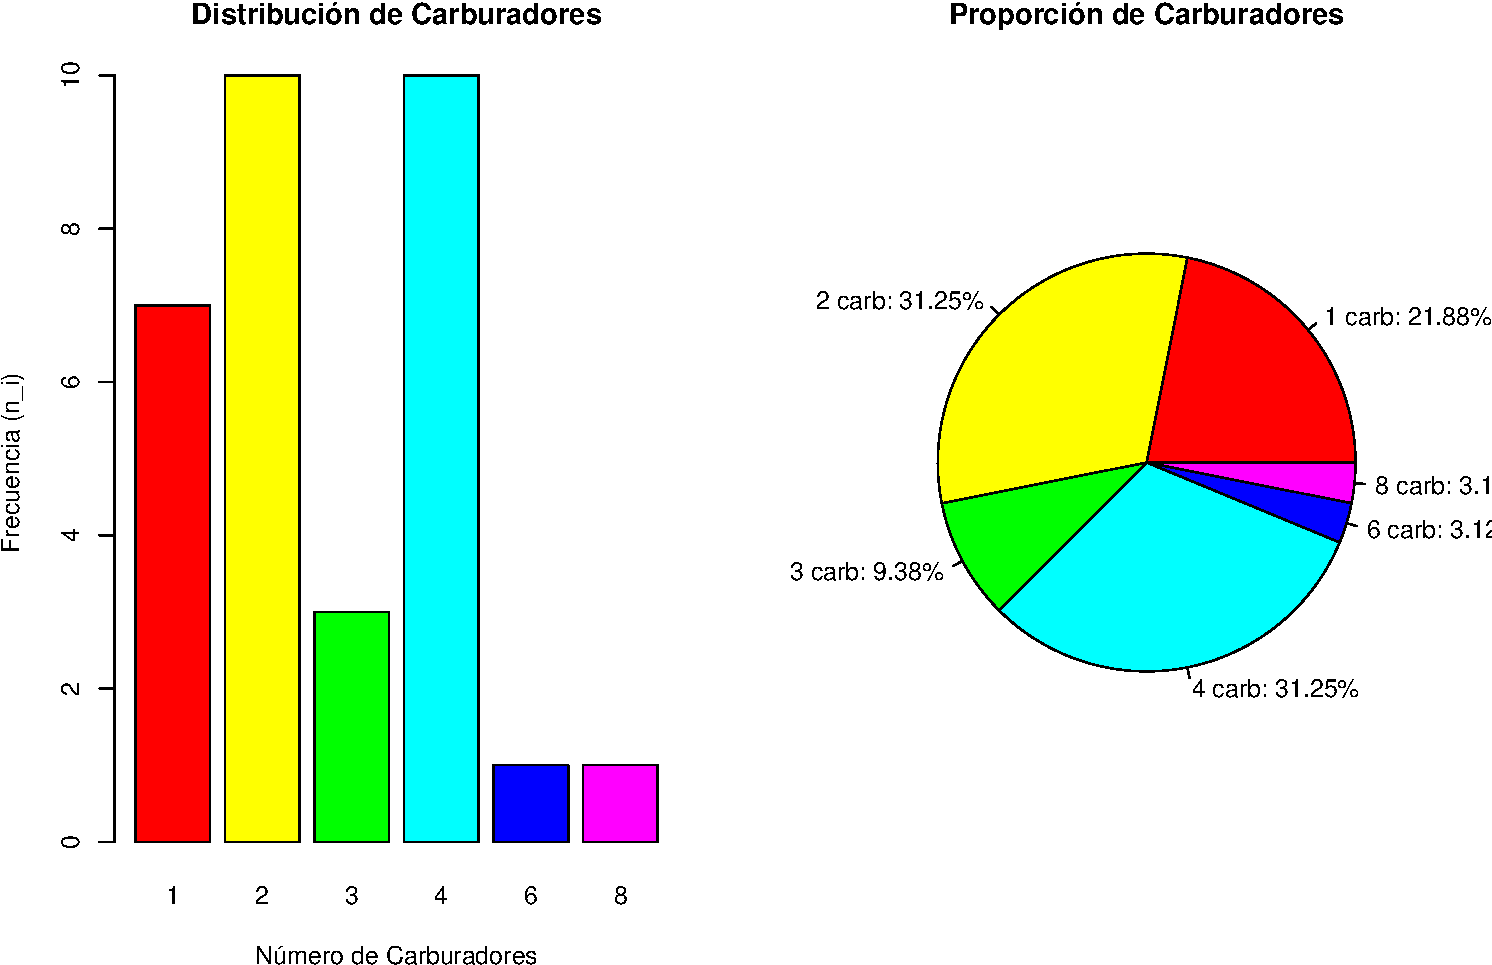
\includegraphics[keepaspectratio]{TablasDeFrecuenciasSimples_files/figure-beamer/unnamed-chunk-7-1.pdf}}
\end{block}
\end{frame}

\begin{frame}[fragile]{Conclusiones I}
\phantomsection\label{conclusiones-i}
\begin{itemize}
\tightlist
\item
  \textbf{Dominio del mercado:} La mayoría de los autos (casi el 63\%)
  tienen 2 o 4 carburadores (sumar los dos valores en la columna
  \texttt{porcentaje}).
\end{itemize}
\end{frame}

\begin{frame}{Conclusiones II}
\phantomsection\label{conclusiones-ii}
\begin{table}
\centering
\caption{\label{tab:unnamed-chunk-8}Tabla de Frecuencias con Resaltado de Análisis}
\centering
\begin{tabular}[t]{c|c|c|c|c|c}
\hline
Carburadores & ni & Ni & fi & Fi & Porcentaje\\
\hline
1 & 7 & 7 & 0.2188 & 0.2188 & 21.88\%\\
\hline
\cellcolor[HTML]{F46D2A}{\textcolor{white}{\textbf{2}}} & \cellcolor[HTML]{F46D2A}{\textcolor{white}{\textbf{10}}} & \cellcolor[HTML]{F46D2A}{\textcolor{white}{\textbf{17}}} & \cellcolor[HTML]{F46D2A}{\textcolor{white}{\textbf{0.3125}}} & \cellcolor[HTML]{F46D2A}{\textcolor{white}{\textbf{0.5312}}} & \cellcolor[HTML]{F46D2A}{\textcolor{white}{\textbf{31.25\%}}}\\
\hline
3 & 3 & 20 & 0.0938 & 0.6250 & 9.38\%\\
\hline
\cellcolor[HTML]{F46D2A}{\textcolor{white}{\textbf{4}}} & \cellcolor[HTML]{F46D2A}{\textcolor{white}{\textbf{10}}} & \cellcolor[HTML]{F46D2A}{\textcolor{white}{\textbf{30}}} & \cellcolor[HTML]{F46D2A}{\textcolor{white}{\textbf{0.3125}}} & \cellcolor[HTML]{F46D2A}{\textcolor{white}{\textbf{0.9375}}} & \cellcolor[HTML]{F46D2A}{\textcolor{white}{\textbf{31.25\%}}}\\
\hline
6 & 1 & 31 & 0.0312 & 0.9688 & 3.12\%\\
\hline
8 & 1 & 32 & 0.0312 & 1.0000 & 3.12\%\\
\hline
\end{tabular}
\end{table}
\end{frame}

\begin{frame}{Conclusiones III}
\phantomsection\label{conclusiones-iii}
\textbf{Rareza:} Los autos con 6 u 8 carburadores son excepciones
(frecuencia absoluta de 1), representando modelos de muy alto
rendimiento para la época.
\end{frame}

\section{Ejercicio para desarrollar en clase con asistencia del
profesor.}\label{ejercicio-para-desarrollar-en-clase-con-asistencia-del-profesor.}

\begin{frame}[fragile]{Ejercicio}
\phantomsection\label{ejercicio}
\begin{tcolorbox}[enhanced jigsaw, opacityback=0, titlerule=0mm, bottomtitle=1mm, colbacktitle=quarto-callout-important-color!10!white, title=\textcolor{quarto-callout-important-color}{\faExclamation}\hspace{0.5em}{Important}, toptitle=1mm, arc=.35mm, breakable, leftrule=.75mm, coltitle=black, toprule=.15mm, colframe=quarto-callout-important-color-frame, left=2mm, rightrule=.15mm, bottomrule=.15mm, colback=white, opacitybacktitle=0.6]

\textbf{Contexto:} Utilizando el mismo dataset \texttt{mtcars}, analicen
ahora la variable \textbf{\texttt{gear} (Número de marchas/cambios hacia
adelante)}.

\end{tcolorbox}
\end{frame}

\begin{frame}{Instrucciones}
\phantomsection\label{instrucciones}
\begin{itemize}
\item
  Identifiquen el número total de observaciones (\(n\)).
\item
  Construyan la tabla de frecuencias completa (clonando la lógica del
  ejemplo anterior).
\item
  Respondan:

  \begin{itemize}
  \item
    ¿Qué porcentaje de los autos tienen 4 marchas? (\(f_i\))
  \item
    ¿Cuántos autos tienen 4 marchas o menos? (\(N_i\)).
  \end{itemize}
\item
  Realicen un diagrama de barras y comenten cuál es la configuración de
  transmisión más común en esa muestra.
\end{itemize}
\end{frame}

\begin{frame}{Para finalizar}
\phantomsection\label{para-finalizar}
\textbf{Comparar} el gráfico de barras con el de dona o circular.

\begin{itemize}
\tightlist
\item
  ¿En qué caso es más fácil ver la diferencia entre el grupo de 3 y 4
  marchas?
\end{itemize}
\end{frame}

\section{Ejercicio para entregar}\label{ejercicio-para-entregar}

\begin{frame}{Ejercicio para entregar}
\begin{tcolorbox}[enhanced jigsaw, opacityback=0, titlerule=0mm, bottomtitle=1mm, colbacktitle=quarto-callout-important-color!10!white, title=\textcolor{quarto-callout-important-color}{\faExclamation}\hspace{0.5em}{Important}, toptitle=1mm, arc=.35mm, breakable, leftrule=.75mm, coltitle=black, toprule=.15mm, colframe=quarto-callout-important-color-frame, left=2mm, rightrule=.15mm, bottomrule=.15mm, colback=white, opacitybacktitle=0.6]

Se debe entregar formato pdf usando la plantilla proporcionada de Quarto
markdown, subiéndolo a Cintia (y solo a Cintia), la próxima clase que es
el miércoles 4 de marzo.

\end{tcolorbox}
\end{frame}

\begin{frame}{Trabajo Independiente: Análisis de Dietas Experimentales}
\phantomsection\label{trabajo-independiente-anuxe1lisis-de-dietas-experimentales}
\begin{tcolorbox}[enhanced jigsaw, opacityback=0, titlerule=0mm, bottomtitle=1mm, colbacktitle=quarto-callout-important-color!10!white, title=\textcolor{quarto-callout-important-color}{\faExclamation}\hspace{0.5em}{Important}, toptitle=1mm, arc=.35mm, breakable, leftrule=.75mm, coltitle=black, toprule=.15mm, colframe=quarto-callout-important-color-frame, left=2mm, rightrule=.15mm, bottomrule=.15mm, colback=white, opacitybacktitle=0.6]

\textbf{Contexto:} En un estudio biológico, se probaron 4 tipos de
dietas diferentes para observar el crecimiento de sujetos
experimentales. Como analista, debes informar sobre la distribución de
estas dietas en la muestra total para asegurar que el experimento esté
balanceado.

\end{tcolorbox}
\end{frame}

\begin{frame}[fragile]{Preparación de los datos}
\phantomsection\label{preparaciuxf3n-de-los-datos}
Carga el dataset y asigna la variable \texttt{Diet} a un objeto para
trabajar.

\begin{Shaded}
\begin{Highlighting}[]
\FunctionTok{data}\NormalTok{(}\StringTok{"ChickWeight"}\NormalTok{)}
\NormalTok{datos\_dieta }\OtherTok{\textless{}{-}}\NormalTok{ ChickWeight}\SpecialCharTok{$}\NormalTok{Diet}
\end{Highlighting}
\end{Shaded}
\end{frame}

\begin{frame}[fragile]{Construcción de la Tabla de Frecuencias}
\phantomsection\label{construcciuxf3n-de-la-tabla-de-frecuencias}
Completa el siguiente bloque para generar la tabla completa. Recuerda
que los resultados deben ser precisos.

\begin{Shaded}
\begin{Highlighting}[]
\CommentTok{\# Calcula las frecuencias siguiendo la lógica de las diapositivas (pág. 7{-}10)}
\NormalTok{ni\_dieta }\OtherTok{\textless{}{-}} \FunctionTok{table}\NormalTok{(datos\_dieta) }\CommentTok{\# Frecuencia Absoluta}
\NormalTok{Ni\_dieta }\OtherTok{\textless{}{-}} \FunctionTok{cumsum}\NormalTok{(ni\_dieta) }\CommentTok{\# Frecuencia Absoluta Acumulada }
\NormalTok{fi\_dieta }\OtherTok{\textless{}{-}} \FunctionTok{prop.table}\NormalTok{(ni\_dieta) }\CommentTok{\# Frecuencia Relativa}
\NormalTok{Fi\_dieta }\OtherTok{\textless{}{-}} \FunctionTok{cumsum}\NormalTok{(fi\_dieta)  }\CommentTok{\# Frecuencia Relativa Acumulada}
\end{Highlighting}
\end{Shaded}
\end{frame}

\begin{frame}[fragile]{Organiza la tabla final}
\phantomsection\label{organiza-la-tabla-final}
\begin{Shaded}
\begin{Highlighting}[]
\NormalTok{tabla\_dieta }\OtherTok{\textless{}{-}} \FunctionTok{data.frame}\NormalTok{(}
  \AttributeTok{Dieta =} \FunctionTok{names}\NormalTok{(ni\_dieta),}
  \AttributeTok{ni =} \FunctionTok{as.vector}\NormalTok{(ni\_dieta),}
  \AttributeTok{Ni =} \FunctionTok{as.vector}\NormalTok{(Ni\_dieta),}
  \AttributeTok{fi =} \FunctionTok{round}\NormalTok{(}\FunctionTok{as.vector}\NormalTok{(fi\_dieta), }\DecValTok{4}\NormalTok{),}
  \AttributeTok{Fi =} \FunctionTok{round}\NormalTok{(}\FunctionTok{as.vector}\NormalTok{(Fi\_dieta), }\DecValTok{4}\NormalTok{),}
  \AttributeTok{Porcentaje =} \FunctionTok{paste0}\NormalTok{(}\FunctionTok{round}\NormalTok{(}\FunctionTok{as.vector}\NormalTok{(fi\_dieta) }\SpecialCharTok{*} \DecValTok{100}\NormalTok{, }\DecValTok{2}\NormalTok{), }\StringTok{"\%"}\NormalTok{)}
\NormalTok{)}
\NormalTok{knitr}\SpecialCharTok{::}\FunctionTok{kable}\NormalTok{(tabla\_dieta, }\AttributeTok{caption =} \StringTok{"Distribución de Frecuencias: Tipos de Dieta"}\NormalTok{)}
\end{Highlighting}
\end{Shaded}
\end{frame}

\begin{frame}[fragile]{Visualización Personalizada}
\phantomsection\label{visualizaciuxf3n-personalizada}
Genera el diagrama de barras aplicando la \textbf{Regla de
Personalización Cromática} (según la letra con que inicia tu nombre).

\begin{Shaded}
\begin{Highlighting}[]
\CommentTok{\# Escribe aquí el código para el barplot con tu color asignado}
\CommentTok{\# No olvides los títulos de los ejes y el título principal}
\end{Highlighting}
\end{Shaded}
\end{frame}

\begin{frame}{Interpretación y Conclusiones}
\phantomsection\label{interpretaciuxf3n-y-conclusiones}
Responda de forma detallada (mínimo 3 párrafos):

\begin{enumerate}
\item
  ¿Cuál es la dieta que más sujetos recibió? Indique su frecuencia
  absoluta (\(n_i\)).
\item
  ¿Qué proporción del total representan las dietas 1 y 2 juntas? (Use
  las frecuencias relativas para el cálculo) .
\item
  Si el investigador afirma que las dietas están repartidas de forma
  equitativa, ¿apoyan sus datos esta afirmación? Justifique su respuesta
  basándose en la tabla.
\end{enumerate}
\end{frame}




\end{document}
